\documentclass[a4paper]{book} %{article}

\usepackage{fullpage} % Package to use full page
\usepackage{parskip} % Package to tweak paragraph skipping
\usepackage{tikz} % Package for drawing
\usepackage{amsmath}
\usepackage{hyperref}
\usepackage[numbered]{bookmark} % For numbering of challenges in bookmark pane of PDF viewer
\def\UrlBreaks{\do\/\do-}
\usepackage[absolute]{textpos}
\setlength{\TPHorizModule}{1mm}
\setlength{\TPVertModule}{1mm}
\usepackage{tikz}
\usepackage{siunitx}
\usepackage{datetime} % Time
\usepackage[UKenglish]{isodate}
\usepackage{ctable} % Thick table lines
\usepackage{booktabs} % Merge cells with multicolumn
\usepackage{bm} % Bold-maths \bm command

\newcommand{\disctime}{13:00 to 14:30 }
\newcommand{\discdays}{Mondays }
\newcommand{\discroom}{W4-766}
%\newcommand{\discexam}{10th February 2017}
\newcommand{\course}{Mechanics }
\newcommand{\courseurl}{mechanics}
\newcommand{\nensei}{2nd}

\newcommand{\lap}[1]{\mathcal{L}\{#1\}}

\newcommand{\six}[1]{\SI[parse-numbers=false]{X}{#1}}
\newcommand{\hash}[2]{MD5(#1\_X) = #2\ldots}
\newcommand{\com}[1]{\overline{#1}}

\graphicspath{{Images/}}

\begin{document}

\begin{titlepage}
    \begin{center}
        \vspace*{1cm}

        \Huge
        \textbf{Mechanics}

        Spring 2017

        \vspace{1.5cm}
        \Large
        Last updated:\\\today \ at \currenttime

        \vspace{4.0cm}
        \LARGE
        James Cannon\\Kyushu University
        \vfill

        \normalsize
        \url{http://www.jamescannon.net/teaching/\courseurl}\\
        \vspace{0.3cm}
        \small
        \url{http://raw.githubusercontent.com/NanoScaleDesign/Mechanics/master/mechanics.pdf}
        \vspace{0.5cm}

        License: \emph{CC BY-NC 4.0}.

    \end{center}
\end{titlepage}

\setcounter{chapter}{-1}

\tableofcontents

\chapter{Course information}
\newpage
\section{This course}
This is the Spring 2017 \course course studied by \nensei-year undegraduate international students at Kyushu University.

\subsection{What you need to do}
\begin{itemize}
    \item Borrow the book ``Engineering Mechanics: Dynamics'', 6th edition, by Meriam and Kraige from the Kikan-kyoiku office in the centre-zone. The course will be based on that book and you will need to refer to it in class.
    \item Prepare a challenge-log in the form of a workbook or folder where you can clearly write the calculations you perform to solve each challenge. This will be used in the final assessment and will be occasionally reviewed by the teacher.
    \item Submit a weekly feedback form by \textbf{9am on Monday} before class at \url{https://goo.gl/forms/2PgFF0eqTOvbK0to2}.
    \item Please bring a wifi-capable internet device to class, as well as headphones if you need to access online components of the course during class. If you let me know in advance, I can lend computers and provide power extension cables for those who require them (limited number).
\end{itemize}

\subsection{How this works}
\begin{itemize}
    \item This booklet forms part of an active-learning segment in the course. The learning is self-directed in contrast to the traditional lecture-style model.
    \item Learning is guided through solving a series of challenges combined with instant feedback about the correctness of your answer.
    \item Traditional lectures are replaced by discussion time. Here, you are encouraged to discuss any issues with your peers, teacher and any teaching assistants. You can also learn from explaining concepts to your peers.
    \item Discussion-time is from \disctime on \discdays at room \discroom.
    \item Peer discussion is encouraged, however, if you have help to solve a challenge, always make sure you do understand the details yourself. You will need to be able to do this in an exam environment. The questions on the exam will be similar in nature to the challenges. If you can do all of the challenges, you can get 100\% on the exam.
    \item Every challenge in the book typically contains a \textbf{Challenge} with suggested \textbf{Resources} which you are recommended to utilise in order to solve the challenge. \textbf{Solutions} will be given. Occasionally the teacher will provide extra \textbf{Comments} to help guide your thinking.
    \item For deep understanding, it is recommended to study the suggested resources beyond the minimum required to complete the challenge.
    \item The challenge document has many pages and is continuously being developed. Therefore it is advised to view the document on an electronic device rather than print it. The date on the front page denotes the version of the document. You will be notified when the document is updated.
    \item A target challenge will be set each week. This will set the pace of the course and define the examinable material. It's ok if you can't quite reach the target challenge for a given week, but you should be careful not to fall behind, since the date of the exam cannot be delayed.
\end{itemize}

\subsection{Assessment}
In order to prove to outside parties that you have learned something from the course, we must perform summative assessments. Details will be released at a later date, but will include your answers to the challenges and a final exam, so be sure to keep a record showing how you calculated the answers to all the challenges.

\newpage
\section{Timetable}

\begin{center}
    \begin{tabular}{|c|c|c|c|}
        \hline
        & \textbf{Discussion} & \textbf{Target} & \textbf{Note}          \\ \specialrule{.1em}{.05em}{.05em}
        \textbf{1}  & 10 April & -            &                          \\ \hline
        \textbf{2}  & 17 April & 1.4          &                          \\ \hline
        \textbf{3}  & 24 April & 1.7          &                          \\ \specialrule{.1em}{.05em}{.05em}    % 1.8 (rotation)
        \textbf{4}  & 8 May    & 1.12         &                          \\ \hline                              % momentum and other problems
        \textbf{5}  & 15 May   & 1.17         &                          \\ \hline                              % 4/6 part I (steady mass flow)
        \textbf{6}  & 22 May   &              &                          \\ \hline                              % 4/6 part II
        \textbf{7}  & 29 May   &              &                          \\ \specialrule{.1em}{.05em}{.05em}    % 4/7 part I (variable mass)
        \textbf{8}  & 5 June   &              &                          \\ \hline                              % 4/7 part II
        \textbf{9}  & 12 June  &              & Mid-term exam            \\ \hline                              % Mid-term exam?
        \textbf{10} & 19 June  &              &                          \\ \hline                              % Kinematics (7/2-7/5)
        \textbf{11} & 26 June  &              &                          \\ \specialrule{.1em}{.05em}{.05em}    % Kinematics general motion (7/6)
        \textbf{12} & 3 July   &              &                          \\ \hline
        \textbf{13} & 10 July  &              &                          \\ \hline
        \textbf{14} & 13 July  &              &                          \\ \hline                              % Legrange
        \textbf{15} & 24 July  & -            & Final exam               \\ \hline
    \end{tabular}
\end{center}


\chapter{Kinetics of systems of particles}
\newpage
\section{System centre-of-mass position, mass and velocity: I}

\subsection*{Resources}
\begin{itemize}
    \item Book sections 4/1 to 4/2
\end{itemize}


\subsection*{Comment}
You may use the following text as an alternative explanation to that in the book.

\subsubsection{Introduction}
You are already largely familiar with the kinetics of a single particle.
The idea of this short course is to extend these principles to the motion of a general system of particles.
This will enable you to describe the motion of both rigid and non-rigid bodies and systems.

A rigid body is defined as a solid system of particles where the distance between the particles does not change with respect to time.
Examples of rigid-bodies are numerous, including many machines operating in the air, on land or under the sea, including rockets and spacecraft.
A non-rigid body can come in two forms:
\begin{itemize}
    \item A single solid body that changes shape over time, perhaps due to elastic or non-elastic deformations.
    \item A defined mass of liquid or gaseous particles flowing at a given rate. Important examples include air and fuel flowing through the turbine of an aircraft engine, the exhaust from the nozzle of a rocket, or water passing through a pump.
\end{itemize}

\subsubsection{Generalising Newton's 2nd law}
Here we extend Newton's second law of motion to cover a general mass system, modelled by considering $n$ particles each with mass $m_i$ bounded by a closed surface in space:

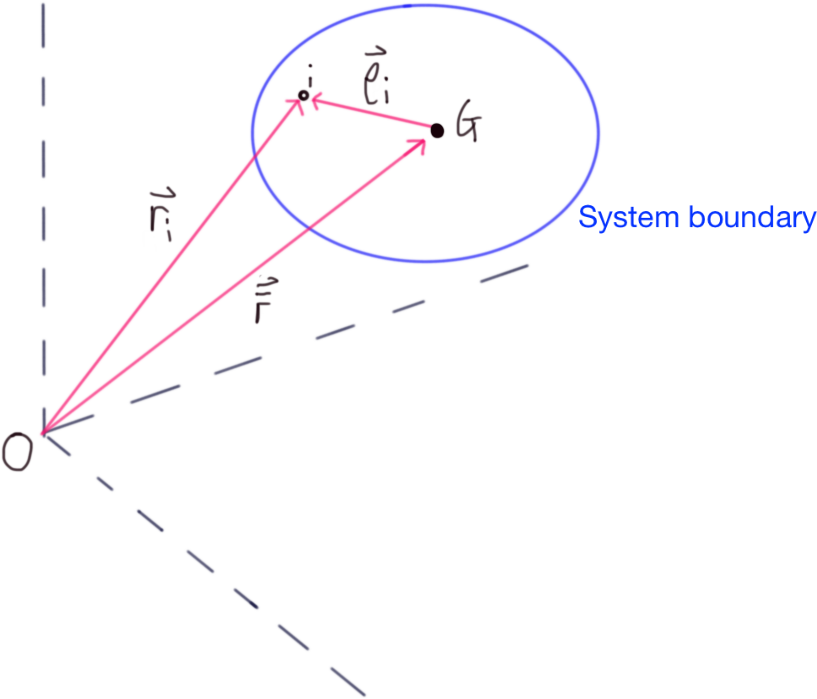
\includegraphics[width=8cm]{particle_system}

The centre-of-mass of the system is denoted by the point $G$ and the distance of particle $i$ from the centre-of-mass is $\bm{\rho_i}$. The distance of particle $i$ from an arbitrary non-accelerating origin $O$ of a Newtonian set of reference axes is $\bm{r_i}$ and the distance of the centre-of-mass from this origin is $\bm{\bar{r}}$. Note that point $G$ does not have to correspond to the position of any one particle, and may just represent the position of the centre-of-mass of the particles at that particular instant.

The total mass of the system $m$ is of course just sum of all the particle masses $m_i$:
\begin{equation}
    m = \sum{m_i}
\end{equation}

so that the centre-of-mass $G$ of the system can be determined from the position of all particles:
\begin{equation}
    m \bm{\bar{r}} = \sum m_i \bm{r}_i
\end{equation}

Each particular in the system is subject to forces. It is useful to group these forces into two contributions:
\begin{itemize}
    \item Sources internal to the system boundary (ie, other particles). For example, the force on particle $i$ by particle $j$.
    \item Sources external to the system boundary (eg, electric fields, gravity, etc).
\end{itemize}

One can consider the total force acting on the system as a whole. Note that the force on on particle $i$ by particle $j$ is equal and opposite to the force on particle $j$ by particle $i$. Thus the sum of forces from internal forces must all cancel out to be zero. If there are multiple external forces $\bm{F}_i$ on the system, then the total force on the system must be $\sum\bm{F}$. Thus the equation of motion for the system can be written as
\begin{equation}
    \label{eqn:generalnewton}
    \sum\bm{F} = m \bm{\bar{\ddot{r}}} = m \bm{\bar{a}}
\end{equation}
where $\bm{\bar{a}}$ corresponds to the acceleration of the centre-of-mass $G$.

Equation \ref{eqn:generalnewton} is the generalised form of Newton's second law of motion. Each component in a Cartesian system may be treated independently (eg, $\sum F_x = m \bar{a}_x$ etc). The resultant external force $\sum\bm{F}$ will have the same direction as the acceleration of the system $\bm{\bar{a}}$ at that instant of time, however the resultant external force does not necessarily pass through the centre-of-mass (usually it does not).


\subsection*{Challenge}
1. $\bm{\com{r}}$, $\dot{\bm{\com{r}}}$ and $\ddot{\bm{\com{r}}}$ of Question 4/1.

2. Question 4/4.

\subsection*{Solution}
1. Given in book.

2. \SI{534}{N}




\newpage
\section{System centre-of-mass position, mass and velocity: II}

\subsection*{Resources}
\begin{itemize}
    \item Book sections 4/1 to 4/2
\end{itemize}

\subsection*{Challenge}
Question 4/5. Determine the \emph{magnitude} of the acceleration.

\subsection*{Solution}
\SI{4}{m/s^2}




\newpage
\section{System centre-of-mass position, mass and velocity: III}

\subsection*{Resources}
\begin{itemize}
    \item Book sections 4/1 to 4/2
\end{itemize}

\subsection*{Challenge}
Question 4/13

\subsection*{Solution}
\SI{4.2}{m/s^2}




\newpage
\section{Kinetic and potential energy}

\subsection*{Resources}
\begin{itemize}
    \item Book section 4/3
\end{itemize}

\subsection*{Challenge}
1. Calculate $T$ in question 4/1

2. Question 4/10

\subsection*{Solution}
1. Given in book.

2. To check your final answer, substitute b = 2 metres into your final answer. You should obtain \SI{5.27}{m/s}.



\newpage
\section{Cross-product}

\subsection*{Resources}
\begin{itemize}
    \item \url{https://www.khanacademy.org/science/physics/magnetic-forces-and-magnetic-fields/electric-motors/v/calculating-dot-and-cross-products-with-unit-vector-notation}
\end{itemize}


\subsection*{Challenge}
1. Determine the angle between the two vectors $\bm{a} = [3,0,0]$ and $\bm{b} = [3,1,0]$ and use it to calculate $\bm{c} = \bm{a} \times \bm{b}$. Which direction does the vector $\bm{c}$ point?

2. Determine the cross product $\bm{f} = \bm{d} \times \bm{e}$ where $\bm{d} = 4 \hat{i}+ 2 \hat{j} + 1 \hat{k}$ and $\bm{e} = -2 \hat{i} -4 \hat{j} + 8 \hat{k}$ without calculating the angle between them.

\subsection*{Solution}
Please compare your answer with your partner and discuss in class if answers differ.




\newpage
\section{Rotation of particles I}

\subsection*{Resources}
\begin{itemize}
    \item Book section 4/4
\end{itemize}

\subsection*{Challenges}
Calculate the angular momentum and the rate of change of angular momentum with time for Question 4/1.

\subsection*{Solutions}
Given in book.



\newpage
\section{Rotation of particles II}

\subsection*{Resources}
\begin{itemize}
    \item Book section 4/4
\end{itemize}

\subsection*{Challenges}
Question 4/15

\subsection*{Solutions}
Given in book.




\newpage
\section{Rotation of particles III}

\subsection*{Resources}
\begin{itemize}
    \item Book section 4/4
\end{itemize}

\subsection*{Challenges}
Question 4/16

\subsection*{Solutions}
The required time should be \SI{2.72}{s}




\newpage
\section{Rotation of particles IV}

\subsection*{Resources}
\begin{itemize}
    \item Book section 4/4
\end{itemize}

\subsection*{Challenges}
Question 4/2

\subsection*{Solutions}
To check your answers substitute $d=2$ metres, $m=7$ kg, $v=3$ m/s and $f=7$ N into your final answers.
You should obtain
$\bm{H}_G = 432 \hat{i} + 144 \hat{j} + 168 \hat{k}$ \SI{}{kg m^2 /s}
and
$\dot{\bm{H}}_G = -8 \hat{i} - 12 \hat{j} + 0 \hat{k}$ \SI{}{Nm}




%\newpage
%\section{Conservation of momentum}
%
%\subsection*{Resources}
%\begin{itemize}
%    \item Book section 4/5
%\end{itemize}
%
%\subsection*{Challenges}
%1. In Question 4/17, at what point does the vehicle stop accelerating? % NT: Change this to calculating velocity first. Add a question about conservation of KE and PE before as well
%
%2. Solve Question 4/17
%
%3. Question 4/18
%
%\subsection*{Solutions}
%1. Please write your answer and compare with your partner in class
%
%2. Given in book
%
%3. 0.21 m/s




%\newpage
%\section{Conservation of momentum vs energy}
%
%\subsection*{Resources}
%\begin{itemize}
%    \item Book section 4/5
%\end{itemize}
%
%\subsection*{Challenges}
%1. Solve Question 4/19
%
%2. Why is energy not conserved here? Where did the energy go? Under what conditions is momentum conserved, and under what conditions is energy conserved?
%
%\subsection*{Solutions}
%1. Given in book
%
%2. Please write your answers and compare with your partner in class.




\newpage
\section{Energy and Rotation I}

\subsection*{Resources}
\begin{itemize}
    \item Book section 4/1 to 4/5
\end{itemize}

\subsection*{Challenge}
Solve Question 4/22.

\subsection*{Solution}
\SI{4.7}{m/s}



\newpage
\section{Energy and Rotation II}

\subsection*{Resources}
\begin{itemize}
    \item Book section 4/1 to 4/5
\end{itemize}

\subsection*{Challenge}
Solve Question 4/28

\subsection*{Solutions}
You should obtain an algebraic expression for $v$ and $\dot{\theta}$. To check your expression, you can substitute the following values into the expression:
$m_0=$ \SI{1}{\kg},
$v_0=$ \SI{1000}{\meter\per\second},
$b=$ \SI{1.5}{\meter} and
$m=$ \SI{4}{\kg}, whereby you should obtain
$v=$ \SI{111}{\meter\per\second} and
$\dot{\theta}=$ \SI{222}{\radian\per\second}.




%\newpage
%\section{In-plane flow}
%
%\subsection*{Resources}
%\begin{itemize}
%    \item Book section 4/6
%\end{itemize}
%
%\subsection*{Challenge}
%Derive equation 4/19 in the book from equation 4/19a.




%\newpage
%\section{Force on vane}
%
%\subsection*{Resources}
%\begin{itemize}
%    \item Book section 4/6
%\end{itemize}
%
%\subsection*{Challenge}
%Show your working for sample problem 4/5 (a) and (b)




%\newpage
%\section{Power and a vane}
%
%\subsection*{Resources}
%\begin{itemize}
%    \item Book section 4/6
%\end{itemize}
%
%\subsection*{Challenge}
%Considering sample problem 4/6,
%
%1. Explain in words what is meant by ``power by action of the fluid''.
%
%2. The power is defined here by measuring the force applied to move an object at a constant velocity. If force creates acceleration ($F=ma$), how can the velocity be constant?
%
%3. Work through and solve the sample problem.
%
%\subsection*{Solutions}
%Please compare your solutions with your partner. You may be asked to present your solutions to the class.




%\newpage
%\section{Balancing forces: Jet aeroplane example}
%
%\subsection*{Resources}
%\begin{itemize}
%    \item Book section 4/6
%\end{itemize}
%
%\subsection*{Challenge}
%Work through sample problem 4/8 to obtain the equation of motion of the system as given in the book ($m'_gu-m'_av=mg\sin{\theta}+D$).




%\newpage
%\section{Balancing forces: Jet aeroplane}
%
%\subsection*{Resources}
%\begin{itemize}
%    \item Book section 4/6
%\end{itemize}
%
%\subsection*{Challenge}
%Answer question 4/33.
%
%\subsection*{Solution}
%Given in book.



%\newpage
%\section{Balancing forces: Fire tug}
%
%\subsection*{Resources}
%\begin{itemize}
%    \item Book section 4/6
%\end{itemize}
%
%\subsection*{Challenge}
%Answer question 4/37.
%
%\subsection*{Solution}
%Given in book.




%\newpage
%\section{Balancing ball on a water stream}
%
%\subsection*{Resources}
%\begin{itemize}
%    \item Book section 4/6
%\end{itemize}
%
%\subsection*{Challenge}
%Answer question 4/42. Take note about the conservation of energy in the jet stream, and the fact that the jet stream remains intact. You can assume that the water stream is fully deflected horizontally when it hits the ball.
%
%\subsection*{Solution}
%\SI{4.8}{\meter}




%\newpage
%\section{Pressure I}
%
%\subsection*{Resources}
%\begin{itemize}
%    \item Book section 4/6
%\end{itemize}
%
%\subsection*{Challenge}
%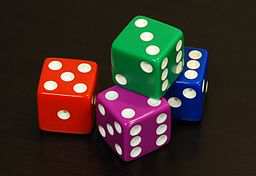
\includegraphics[width=4cm]{dice}
%
%A typical die has a side length of \SI{1.4}{\cm} and weighs \SI{2.8}{\gram}. Consider the die at rest on a desk. Estimate the pressure on the bottom of the die due to the desk.
%
%\subsection*{Solution}
%\SI{140}{\pascal}




%\newpage
%\section{Pressure II}
%
%\subsection*{Resources}
%\begin{itemize}
%    \item Book section 4/6
%\end{itemize}
%
%\subsection*{Challenge}
%Answer question 4/50
%
%\subsection*{Solution}
%\SI{1035}{\pascal}




%\newpage
%\section{Hose}
%
%\subsection*{Resources}
%\begin{itemize}
    %\item Book section 4/6
%\end{itemize}
%
%\subsection*{Challenge}
%Consider question 4/62. Note that the volume flow rate $Q$, measured in $m^3/s$, is the total system volume flow rate, and therefore the volume flow rate emerging from each nozzel is one quater of this for each nozzel.
%
%1. Write an expression for the velocity parallel and perpendicular to rotation for the case where $b$ tends to zero.
%
%2. Write an expression for the velocity parallel and perpendicular to rotation for the case where $r$ tends to zero.
%
%3. Remembering that components of angular velocity can be combined linearly independently, write an expression for the velocity parallel and perpendicular to rotation for the case where neither $b$ or $r$ are tending to zero.
%
%Answer question 4/62
%
%\subsection*{Solution}



%\newpage
%\section{Power and a Helicopter}
%
%\subsection*{Resources}
%\begin{itemize}
%    \item Book section 4/6
%\end{itemize}
%
%\subsection*{Challenge}
%Answer question 4/59
%
%\subsection*{Solutions}
%Given in book




%\newpage
%\section{Force components}
%
%\subsection*{Resources}
%\begin{itemize}
%    \item Book section 4/6
%\end{itemize}
%
%\subsection*{Challenge}
%Answer question 4/61
%
%\subsection*{Solutions}
%Given in book




\newpage
\section{Mass ejection}

\subsection*{Resources}
\begin{itemize}
    \item Book section 4/7
\end{itemize}

\subsection*{Challenge}
Consider rocket thrust where exhaust is emitted at a speed of \SI{220}{\meter\per\second}. The force on the rocket due to the thrust alone is \SI{400}{\newton}. Calculate (a) the mass flow rate $m'$ and (b) the time-rate increase of the mass of the rocket $\dot{m}$.

\subsection*{Solutions}
(a)\\
\soltwodp{a}{b54e89} (\SI{}{\kg\per\second})

(b)\\
\soltwodp{b}{6a83d8} (\SI{}{\kg\per\second})




\newpage
\section{Rocket sample problem}

\subsection*{Resources}
\begin{itemize}
    \item Book section 4/7
\end{itemize}

\subsection*{Challenge}
Complete the sample problem 4/11 using both solution I and II. Please be sure to follow the logic and understand the link between the two methods.




\newpage
\section{Rocket-style problem I}

\subsection*{Resources}
\begin{itemize}
    \item Book section 4/7
\end{itemize}

\subsection*{Challenge}
Answer question 4/67

\subsection*{Solution}
Given in book.




\newpage
\section{Rocket-style problem II}

\subsection*{Resources}
\begin{itemize}
    \item Book section 4/7
\end{itemize}

\subsection*{Challenge}
Answer question 4/82

\subsection*{Solution}
\SI{4.8}{\meter\per\second}




\newpage
\section{Mass intake I}

\subsection*{Resources}
\begin{itemize}
    \item Book section 4/7
\end{itemize}

\subsection*{Challenge}
Answer question 4/80

\subsection*{Solution}
\SI{1.6}{\meter\per\square\second} deceleration




\newpage
\section{Mass intake II}

\subsection*{Resources}
\begin{itemize}
    \item Book section 4/7
\end{itemize}

\subsection*{Challenge}
Answer question 4/76

\subsection*{Solution}
\SI{0.152}{\meter\per\square\second}




\newpage
\section{Chain style sample problem}

\subsection*{Resources}
\begin{itemize}
    \item Book section 4/7
\end{itemize}

\subsection*{Challenge}
Work through sample problem 4/9




\newpage
\section{Rope style sample problem}

\subsection*{Resources}
\begin{itemize}
    \item Book section 4/7
\end{itemize}

\subsection*{Challenge}
Work through sample problem 4/10




\newpage
\section{Chain vs Rope style sample problem difference}

\subsection*{Resources}
\begin{itemize}
    \item Book section 4/7
\end{itemize}

\subsection*{Challenge}
Considering the chain sample problem and the unconstrained rope problem, why was the kinetic energy different in these two cases? What assumptions were made in the chain problem compared to the unconstrained rope problem, and how did this impact the calculation of kinetic energy?

Please write a few sentences summarising your understanding.

\subsection*{Solution}
Please compare your writing with your partner's writing and discuss any differences.




\newpage
\section{Constrained and unconstrained rope style sample problem}

\subsection*{Resources}
\begin{itemize}
    \item Book section 4/7
\end{itemize}

\subsection*{Challenge}
Considering the unconstrained and constrained rope sample problem, how are the approaches different? How do the different values for ``P'' and ``R'' arise? What assumptions are different?

Please write a few sentences summarising your understanding.

\subsection*{Solution}
Please compare your writing with your partner's writing and discuss any differences.



\newpage
\section{Lifting a chain}

\subsection*{Resources}
\begin{itemize}
    \item Book section 4/7
\end{itemize}

\subsection*{Challenge}
An 18K gold chain has a mass of \SI{1.12}{\gram} and a length of \SI{40}{\cm}. You pick up one end of the chain and lift it up vertically at a constant velocity. There will be two downward forces present: one due to the hanging weight of the chain due to earth's gravity ($A$), and another induced by the constant addition of mass to the hanging part of the chain ($B$). If the chain is lifted up at \SI{5}{\cm\per\s}, calculate $B$. State what simplifying assumptions you make. How does this compare to $A$?

\subsection*{Solution}
$B$: \SI{7}{\micro\newton}




\newpage
\section{Chain on a pully}

\subsection*{Resources}
\begin{itemize}
    \item Book section 4/7
\end{itemize}

\subsection*{Challenge}
Answer question 4/83

\subsection*{Solution}
$P$ is given in book, and $R$ should match your understanding of the weight of the pile.




\newpage
\section{An accelerating chain}

\subsection*{Resources}
\begin{itemize}
    \item Book section 4/7
\end{itemize}

\subsection*{Challenge}
\textbf{a)} Consider a chain hanging over the edge of a block of height $h$. The chain has a total length $L$ and mass per unit length of $\rho$. At time t=0, the right end of the chain lays on top of the block at its right side at position x=0, while the left end of the chain is barely touching the ground. Initially the chain is stationary, but then the chain is released, causing the right side to accelerate horizontally in the left direction and the chain to pile up to the left of the block. Ignoring friction at the corner and making other idealised assumptions, obtain an expression for the acceleration of the chain as a function of the position of the end of the chain ($x$) as it slides along the horizontal surface, before it reaches the end of the block.

\textbf{b)} Did you need to consider the force generated by the stopping of the chain as it landed on the ground? If so, how did it come into the equation? If not, why not?

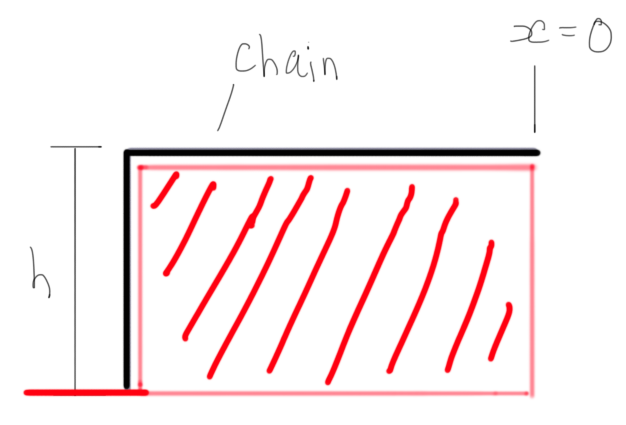
\includegraphics[height=5cm]{sliding_chain}

\subsection*{Solution}
\textbf{a)} To check your answer, determine the acceleration for a height of \SI{5}{\meter} and chain length of \SI{10}{\meter}, when the chain has slid \SI{2}{m}. You should obtain an acceleration of \SI{6.13}{\meter\per\square\second}.

\textbf{b)} Please discuss your answer with your partner



\newpage
\section{Making a question}

\fbox{\textbf{Coursework challenge}}

\subsection*{Resources}
\begin{itemize}
    \item Book section 4
\end{itemize}

\subsection*{Challenge}
Create an original question concerning anything covered in this chapter using the Peerwise platform (see section \ref{sec:peerwise} for details). If you create more than one question, the question awarded highest marks will be counted.

Your question must contain the following:
\begin{enumerate}
    \item A diagram to support your question.
    \item 5 possible answer options (A-E) that can be used by the student to check if their answer is correct. These may be numerical, mathematical, word-based or hashes.
    \item It is important that it is not possible to derive the method from the answer-options that you give.
    \item All the answer options should be plausible.
    \item For at least one of your wrong-answer options, ensure that the answer corresponds to a typical mistake that a student might make when answering your question. \label{lab:typical}
    \item Provide a detailed solution to your question, including explanation and mathematics. \emph{Demonstrate your own thinking and understanding.}
    \item Related to item \ref{lab:typical}, explain why the student might have chosen that wrong answer, and explain where they may have gone wrong in their thinking.
\end{enumerate}




\newpage
\section{Answering Peerwise question(s)}

\subsection*{Resources}
\begin{itemize}
    \item Book section 4
\end{itemize}

\subsection*{Challenge}
Choose at least one question from Peerwise and attempt to answer it.
Explain your reasoning (don't just write mathematics).
Clearly write an alternative explanation or possible improvement to the question you answered.

\subsection*{Solution}
Please discuss in class.


\end{document}
